% =====================================================================
% Preliminary Report -- Master Computer Science
% "Quantifying Process Model Generalization"
% LNCS / Springer format. Compile with: pdflatex main && bibtex main && pdflatex main && pdflatex main
% (MiKTeX: add -enable-installer on first compile)
% =====================================================================
\documentclass[runningheads]{llncs}

\usepackage[T1]{fontenc}
\usepackage{graphicx}
\usepackage{amsmath}
\usepackage{amssymb}
\usepackage{booktabs}
\usepackage{multirow}
\usepackage{tikz}
\usetikzlibrary{positioning,arrows.meta}
\usepackage[hidelinks]{hyperref}

\newcommand{\genshadow}{\ensuremath{\mathit{Gen}_{\mathit{shadow}}}}
\newcommand{\genaccept}{\ensuremath{\mathit{Gen}_{\mathit{accept}}}}
\newcommand{\punseen}{\ensuremath{p_{\mathit{unseen}}}}
\newcommand{\pend}{\ensuremath{p_{\mathit{end}}}}

\begin{document}

\title{Quantifying Process Model Generalization:\\
A Generative N-gram Metric and a Cross-Paradigm Benchmark\thanks{Preliminary report, Master of Science in Computer Science.}}
\titlerunning{Quantifying Process Model Generalization}

% TODO: fill in author name, institute, and supervisor before submission.
\author{Author Name\inst{1}}
\authorrunning{Author Name}
\institute{Institute, University\\
\email{author@university.example}}

\maketitle

\begin{abstract}
Generalization---the ability of a discovered process model to accept behavior that is valid under the underlying process but absent from the recorded event log---is the least understood of the four established process model quality dimensions. Existing metrics rest on incompatible paradigms, are rarely compared against each other, and are almost never validated against an empirical ground truth. This report makes four contributions. First, we argue for a \emph{strict construct definition}: generalization measures only the acceptance of future valid behavior; penalizing over-permissiveness is the task of precision, and conflating the two destroys the diagnostic value of the quality quadrant. Second, we present \emph{HybridGen}, a generative metric that derives a stochastic trace generator from the event log via variable-order N-gram statistics with Katz-style backoff and Good--Turing novelty estimation, and scores a model by replaying the resulting synthetic \emph{shadow log}. Third, we design a benchmark that confronts our metric, its ablation lineage, and seven published baselines with eight discovery configurations---including a trace model and a flower model as the 0/1 poles of the construct---anchored by variant-based cross-validation as ground truth. Fourth, we report results on two datasets: the current metric version tracks the ground truth at Pearson $0.996$/$0.993$ (MAE $0.023$/$0.022$) while the widely used PM4Py metric correlates \emph{negatively}; an iterative version study shows that two probe defects, once measured, could be repaired with a $3\times$ calibration gain; and a strict \emph{acceptance} reading of the same probe, validated against its own acceptance-based ground truth, anchors both poles exactly.

\keywords{Process mining \and Process discovery \and Generalization \and Model quality \and Conformance checking \and Benchmark.}
\end{abstract}

% =====================================================================
\section{Introduction}
\label{sec:intro}

Process discovery algorithms construct process models from event logs recorded by information systems~\cite{vanderaalst2016pm}. The quality of a discovered model is conventionally assessed along four dimensions: \emph{fitness} (the model can replay the observed behavior), \emph{precision} (the model does not allow much behavior beyond what was observed), \emph{simplicity} (the model is structurally parsimonious), and \emph{generalization}~\cite{buijs2014quality}. Generalization captures the insight that an event log is only a \emph{sample} of the underlying process: a good model should also accept future, not-yet-observed behavior that the process can produce.

Generalization is widely regarded as the most elusive of the four dimensions, for a structural reason: it makes a claim about behavior that, by definition, is not in the data. Existing metrics approach the problem from fundamentally different angles---counting rarely used model parts~\cite{buijs2014quality}, information-theoretic relevance of stochastic models~\cite{alkhammash2022entropic}, adversarial anti-alignments~\cite{vandongen2016anti}, generative adversarial networks~\cite{theis2020avatar}, statistical bootstrapping~\cite{polyvyanyy2022bootstrap}, and biodiversity-inspired species estimation~\cite{kabierski2023species}. These paradigms produce scores that are not obviously commensurable, and to the best of our knowledge no study has systematically compared them against each other \emph{and} against an empirical ground truth on common real-life logs.

This preliminary report documents the current state of a Master's project that addresses this gap. Its contributions are:

\begin{enumerate}
  \item \textbf{A strict construct position.} We define generalization as the acceptance of future \emph{valid} behavior and nothing else (Sect.~\ref{sec:construct}). Two degenerate models operationalize the poles of this construct: a trace model (memorization, low pole) and a flower model (universal acceptance, high pole). Under this definition the flower model \emph{correctly} receives the maximal score---making it a litmus test that separates pure generalization metrics from those contaminated with precision or structural notions.
  \item \textbf{A generative metric.} \emph{HybridGen}\footnote{The name is historical: an earlier design combined the generative score with a structural counterweight. The structural component was retired (Sect.~\ref{sec:method}); the name is kept for continuity with the codebase.} derives a variable-order Markov model from the log (N-grams up to order $N{=}6$, Katz-style backoff~\cite{katz1987}), estimates per-context novelty mass by Good--Turing estimation~\cite{gale1995gt}, generates a synthetic \emph{shadow log} of unseen traces, and scores a model by replaying it (Sect.~\ref{sec:method}).
  \item \textbf{A validated benchmark.} We evaluate the metric's full version lineage (seven configurations, M1--M1f) and seven external baselines across eight discovery configurations on real-life logs, with variant-based $k$-fold cross-validation as empirical ground truth and a three-criterion agreement protocol (rank correlation, calibration error, discriminative spread), because rank correlation alone is a bar that even a random-replay baseline clears (Sect.~\ref{sec:benchmark}--\ref{sec:results}).
  \item \textbf{Measured iteration.} The benchmark exposed two probe defects in earlier metric versions---an implausible mutation proposal and a distribution-distorting sampling weight. Repairing them improved calibration $3\times$ (MAE $0.077 \to 0.023$) and corrected a ranking error on the second dataset; a strict \emph{acceptance} reading of the same probe was added and validated against its own acceptance-based ground truth (Sect.~\ref{sec:results:versions}--\ref{sec:results:accept}).
\end{enumerate}

The remainder is structured as follows: Sect.~\ref{sec:background} introduces preliminaries and related work, Sect.~\ref{sec:construct} states the construct position, Sect.~\ref{sec:method} presents the metric, Sect.~\ref{sec:ngram} summarizes the calibration of the context depth, Sect.~\ref{sec:benchmark} the benchmark design, Sect.~\ref{sec:results} the results, Sect.~\ref{sec:discussion} discussion and threats to validity, and Sect.~\ref{sec:conclusion} the road map.

% =====================================================================
\section{Background and Related Work}
\label{sec:background}

\subsection{Preliminaries}

Let $\mathcal{A}$ be a finite set of \emph{activities}. A \emph{trace} $\sigma \in \mathcal{A}^*$ is a finite sequence of activities; an \emph{event log} $L$ is a multiset of traces; traces with identical activity sequences form a \emph{variant}. A discovery algorithm (\emph{miner}) maps a log to a model; in this work all models are accepting Petri nets discovered with PM4Py~\cite{berti2019pm4py}. \emph{Token replay}~\cite{rozinat2008conformance} replays a trace on a net and returns (i) a graded trace fitness in $[0,1]$ based on produced, consumed, missing, and remaining tokens, and (ii) a Boolean flag whether the trace replays \emph{perfectly}. The distinction matters throughout this report: graded fitness grants \emph{partial credit} to traces the model cannot actually execute end-to-end.

\subsection{Existing Generalization Metrics}
\label{sec:relwork}

We group published metrics by paradigm; identifiers M2--M8 refer to benchmark roles (Sect.~\ref{sec:benchmark}). The PM4Py built-in metric (M2)~\cite{buijs2014quality,berti2019pm4py} counts rarely visited model parts during replay of the observed log; it never confronts the model with unseen behavior. Entropic relevance (M3)~\cite{alkhammash2022entropic} measures the compression cost of a log under a stochastic model. Anti-alignments (M4)~\cite{vandongen2016anti} search for model traces maximally distant from the log; the optimization is exponential. AVATAR (M5)~\cite{theis2020avatar} trains a sequence GAN to approximate the underlying \emph{system} and scores the harmonic mean of fitness and precision against GAN samples---an F-measure against approximated system behavior, a point we return to in Sect.~\ref{sec:construct}. Bootstrap generalization (M6)~\cite{polyvyanyy2022bootstrap} resamples and recombines log traces and aggregates model quality over replicates. SpeciAL (M7)~\cite{kabierski2023species} transfers species-richness estimation from ecology to event data. Pattern-based generalization (M8)~\cite{reissner2020pattern} reads generalization off discovered behavioral patterns.

\subsection{Membership vs.\ Graded Semantics}
\label{sec:membership}

The \emph{definitions} of generalization in the literature are membership-shaped: van der Aalst's formulation---the likelihood that previously unseen but valid behavior is \emph{allowed} by the model~\cite{vanderaalst2016pm}---asks a yes/no question per trace, and the exact-matching school~\cite{alkhammash2022entropic,polyvyanyy2022bootstrap} builds on Boolean language membership. The \emph{practice}, however, is graded: token-based and alignment-based fitness were introduced precisely so that an almost-correct trace does not count the same as noise~\cite{rozinat2008conformance}. As Sect.~\ref{sec:results:accept} shows empirically, the graded convention also hides something: strict acceptance collapses to zero for entire model classes, and partial credit is what keeps their scores afloat. Our metric therefore reports \emph{both} readings of the same probe.

\subsection{Empirical Ground Truth via Cross-Validation}

The most direct operationalization of generalization is hold-out evaluation: discover a model on a subset of the \emph{variants}, then measure how well withheld variants replay. Variant-based $k$-fold cross-validation (R1) and leave-one-variant-out (R2) realize this at increasing granularity. They are expensive---R2 requires one discovery run per variant---and, crucially, they are only \emph{defined} when the model can be rediscovered from log subsets: they evaluate a discovery \emph{algorithm} on a log, not a model artifact in hand. Both points motivate cheap single-shot metrics that are \emph{calibrated against} R1 where it exists and remain applicable where it does not.

% =====================================================================
\section{Construct: What Generalization Is---and Is Not}
\label{sec:construct}

We adopt a strict construct definition: \textbf{generalization is the degree to which a model accepts future, valid behavior of the underlying process that is absent from the log.} Nothing else. In particular, generalization is \emph{not} precision: detecting over-permissiveness---the acceptance of \emph{invalid} behavior---is the precision dimension's task. Folding a permissiveness penalty into a generalization score makes any mid-range value ambiguous (one cannot distinguish ``rejects future valid behavior'' from ``accepts invalid behavior'') and thereby destroys the diagnostic value of the quality quadrant. One does not redefine recall because a degenerate classifier achieves maximal recall; one reports precision next to it. Metrics that blend the two---e.g.\ AVATAR's harmonic mean of fitness and precision, literally an F-measure---measure a legitimate but \emph{different} construct (closeness to the approximated system), and must not be read as pure generalization.

Two degenerate models operationalize the poles:
\begin{itemize}
  \item the \textbf{flower model} (all activities in one loop) accepts every sequence over $\mathcal{A}$; its generalization is maximal \emph{by definition}. It is a useless model because of its precision and simplicity, not its generalization. A pure generalization metric must score it $\approx 1$;
  \item the \textbf{trace model} (one isolated path per observed variant) memorizes the log and accepts nothing unseen; it is the $0$ pole.
\end{itemize}
This yields a \emph{construct-purity litmus}: a metric scoring the flower model below $1$ demonstrably mixes precision or structure into its score. Our benchmark applies this litmus to every method. Intended usage follows directly: the generalization score is to be read \emph{alongside} precision, never alone; a model with $\mathit{Gen} \approx 1$ and precision $\approx 0$ is diagnosed as over-permissive---by the precision column, where that information belongs.

% =====================================================================
\section{The HybridGen Metric}
\label{sec:method}

\subsection{Overview}

HybridGen scores a model by the replay quality of a synthetic \emph{shadow log}: traces generated from a stochastic model of the log that are plausible under the process but, by construction, absent from the log. The generator is derived from the log only; the model under evaluation is consulted exclusively at replay time (Fig.~\ref{fig:pipeline}). An early design combined this generative score with a structural counterweight ($\mathit{Gen}_{\mathit{total}} = w \cdot \genshadow + (1-w)\cdot\mathit{Gen}_{\mathit{struct}}$); the structural component was retired in v2.3---under the construct of Sect.~\ref{sec:construct}, its anti-flower role belongs to precision, and its anti-overfitting role is already covered by replay failures of recombined traces. The current score is the pure generative component.

\begin{figure}[t]
\centering
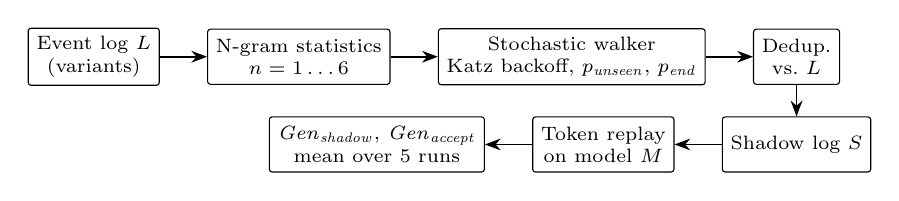
\begin{tikzpicture}[
  node distance=4mm and 6mm,
  box/.style={draw, rounded corners=1pt, align=center, font=\scriptsize, inner sep=3pt, minimum height=7mm},
  arr/.style={-{Stealth[length=2mm]}, semithick}
]
\node[box] (log) {Event log $L$\\(variants)};
\node[box, right=of log] (stats) {N-gram statistics\\$n = 1 \dots 6$};
\node[box, right=of stats] (walk) {Stochastic walker\\Katz backoff, $\punseen$, $\pend$};
\node[box, right=of walk] (dedup) {Dedup.\\vs.\ $L$};
\node[box, below=of dedup] (shadow) {Shadow log $S$};
\node[box, left=of shadow] (replay) {Token replay\\on model $M$};
\node[box, left=of replay] (score) {$\genshadow$, $\genaccept$\\mean over 5 runs};
\draw[arr] (log) -- (stats);
\draw[arr] (stats) -- (walk);
\draw[arr] (walk) -- (dedup);
\draw[arr] (dedup) -- (shadow);
\draw[arr] (shadow) -- (replay);
\draw[arr] (replay) -- (score);
\end{tikzpicture}
\caption{Pipeline (current version, v26). The generator is derived from the log only.}
\label{fig:pipeline}
\end{figure}

\subsection{Shadow Log Generation (v26)}
\label{sec:shadow}

\subsubsection{Variable-order statistics and backoff.}
For every order $n \le N_{\max}$ (default $6$), the generator records per observed $n$-gram context the frequency of each successor activity and the frequency of trace termination, weighted by variant case counts. At generation time the walker resolves each decision at the deepest order whose support meets a threshold $\tau{=}5$, falling back otherwise (Katz-style backoff~\cite{katz1987}). $N_{\max}$ is thus an upper bound; sparse logs degrade gracefully to lower effective orders.

\subsubsection{Novelty: rate and proposal.}
The mutation mechanism has two halves. The \emph{rate}---how often a never-seen continuation occurs after context $s$---is estimated by Good--Turing~\cite{gale1995gt}: $\punseen(s) = N_1(s)/N(s)$, where $N_1$ counts successors observed exactly once. The backoff acts as a safety valve against sparsity-inflated rates. The \emph{proposal}---\emph{which} activity is inserted when a mutation fires---is drawn from the deepest \emph{lower-order} context's successor distribution, restricted to activities unseen at the resolved order: behavior plausible in a related, shorter context but novel in this specific one. This completes the Katz design; earlier versions used a uniform draw over the alphabet, a maximum-entropy placeholder whose cost became measurable only against ground truth (Sect.~\ref{sec:results:versions}). Notably, the mutated share of shadow traces is strongly dataset-dependent: ${\sim}4\,\%$ on BPI 2017 but ${\sim}50\,\%$ on the sparse Sepsis log, where backoff resolves at short contexts with high novelty mass---on such logs the proposal distribution materially shapes the score.

\subsubsection{Exploitation: two sampling modes.}
For non-mutation steps the walker samples a seen successor with probability proportional to either $\ln(f{+}1)$ (\texttt{log} mode, the historical choice, which deliberately up-weights rare paths) or $f$ itself (\texttt{mle} mode, which samples the estimated future-trace distribution and uses the same statistics as the Good--Turing estimate). The two modes answer different questions---expected-future acceptance vs.\ rare-behavior stress test---and Sect.~\ref{sec:results:versions} shows the difference is measurable.

\subsubsection{Termination, deduplication, integrity.}
Trace termination uses a context-dependent probability $\pend(s)$ resolved with the same backoff (correcting premature termination when ``ending activities'' appear early). Every generated trace is checked against the original variant set and regenerated if it is a copy, so the shadow log contains only unseen sequences. Walks are capped at twice the longest observed trace length; truncations and deduplication-cap exhaustions are counted and reported rather than silently absorbed.

\subsubsection{Scoring: two readings of one probe.}
A shadow log of $\min(1000, |L|)$ traces is replayed on the model; generation and replay are repeated five times (all randomness seeded). Two scores are reported: \genshadow, the mean graded trace fitness (the headline score), and \genaccept, the fraction of shadow traces replayed \emph{perfectly}---the strict reading that matches the membership-shaped definition of Sect.~\ref{sec:membership}. Both are additionally stratified into regular vs.\ mutated shadow traces (the \emph{openness profile}).

\subsection{Version Lineage}

Table~\ref{tab:versions} summarizes the evolution; frozen snapshots of each stage enter the benchmark as ablation variants, so every design decision's contribution is measurable in isolation.

\begin{table}[t]
\centering
\caption{Version history; benchmark roles in parentheses.}
\label{tab:versions}
\setlength{\tabcolsep}{4pt}
\footnotesize
\begin{tabular}{@{}llp{6.2cm}@{}}
\toprule
Version & Role & Key change \\
\midrule
v1      & M1a & 1-gram directly-follows generator, Good--Turing mutation \\
v2/v2.1 & M1b ($N{=}3$), M1c ($N{=}6$) & N-gram contexts, Katz backoff, $\ln(f{+}1)$ weights \\
v2.2--v2.3 & --- & structural component added, then retired; deduplication; context-aware $\pend$ \\
v24     & M1  & variant compression, memoization, iterative walker \\
v25     & M1d & Katz-consistent mutation \emph{proposal}; integrity counters \\
v26     & M1e (\texttt{log}), M1f (\texttt{mle}) & acceptance reading \genaccept; data-driven length cap; sampling-mode switch \\
\bottomrule
\end{tabular}
\end{table}

% =====================================================================
\section{Calibrating the Context Order}
\label{sec:ngram}

The maximal order $N_{\max}$ trades context specificity against per-context support. A sweep of $N_{\max}=1,\dots,8$ on BPI Challenge 2017 (Table~\ref{tab:sweep}) shows the realized mutation rate peaking at $N{=}6$ ($49\times$ the 1-gram baseline) and declining beyond, as backoff increasingly rejects sparse contexts---the curse of dimensionality overtaking the context benefit. Backoff counts grow super-linearly after $N{=}5$ while top-order usage collapses below 75\,\%. We therefore fix $N_{\max}{=}6$ \emph{across all datasets}: per-dataset tuning would undermine comparability, and sparse logs are protected by the backoff. Two caveats are recorded honestly: the calibration target (mutation rate) is a proxy, not agreement with ground truth; and it concerns the mutation \emph{rate} half of the mechanism only---the proposal half was revised later (Sect.~\ref{sec:method}) without affecting the rate, so the calibration carries over.

\begin{table}[t]
\centering
\caption{N-gram order sweep on BPI Challenge 2017 (1{,}000 shadow traces, $\tau{=}5$, seed 42).}
\label{tab:sweep}
\setlength{\tabcolsep}{4.5pt}
\footnotesize
\begin{tabular}{@{}lrrrrrrrr@{}}
\toprule
 & $N{=}1$ & $N{=}2$ & $N{=}3$ & $N{=}4$ & $N{=}5$ & $\mathbf{N{=}6}$ & $N{=}7$ & $N{=}8$ \\
\midrule
Mutation rate ($\times 10^{-3}$) & 0.027 & 0.211 & 0.376 & 0.664 & 0.882 & \textbf{1.333} & 1.255 & 1.208 \\
Mutated traces (of 1000)         & 1     & 5     & 12    & 20    & 26    & \textbf{38}    & 37    & 40 \\
Top-order usage (\%)             & 100   & 96.6  & 92.6  & 88.9  & 83.8  & \textbf{80.0}  & 75.5  & 72.4 \\
Backoffs                         & 0     & 111   & 466   & 1{,}128 & 2{,}400 & \textbf{3{,}788} & 5{,}477 & 7{,}514 \\
\bottomrule
\end{tabular}
\end{table}

% =====================================================================
\section{Benchmark Design}
\label{sec:benchmark}

\subsection{Methods, Miners, Datasets}

The benchmark evaluates three tiers: our method's full version lineage (M1, M1a--M1f; Table~\ref{tab:versions}), external baselines spanning all paradigms of Sect.~\ref{sec:relwork} (M2--M8), and reference metrics (R1: variant-based 5-fold CV fitness, 3 shuffles; R2: leave-one-variant-out; R3: replay of uniformly random traces as a floor---a metric scoring a model below random garbage is broken). \emph{Eight} discovery configurations span the construct's poles: a \textbf{filtered trace model} (top-50 variants by frequency; the full trace model with one branch per variant is intractable for replay on variant-rich logs), Alpha, Alpha$+$~\cite{vanderaalst2004alpha}, Heuristics default/strict~\cite{weijters2006hm}, Inductive strict/infrequent~\cite{leemans2013im,leemans2014imf}, and a \textbf{flower model}. Five real-life logs are selected from a profiled 20-log catalog to span trace depth, variant diversity, scale, and repetitiveness (Table~\ref{tab:datasets}); D1 is fully evaluated across all tiers, D2 for the M1 family and ground truth, D3--D5 are scheduled (Sect.~\ref{sec:conclusion}).

\begin{table}[t]
\centering
\caption{Benchmark datasets. TLRA $= 1 - |\text{variants}|/|\text{cases}|$.}
\label{tab:datasets}
\setlength{\tabcolsep}{2.2pt}
\footnotesize
\begin{tabular}{@{}llrrrrrl@{}}
\toprule
ID & Log & Cases & Events & Variants & Avg.\ len & TLRA & Status \\
\midrule
D1 & Sepsis~\cite{mannhardt2016sepsis} & 1{,}050 & 15{,}214 & 846 & 14.5 & 0.19 & all tiers \\
D2 & BPI 2013 Incidents & 7{,}554 & 65{,}533 & 1{,}511 & 8.7 & 0.80 & M1 family + R1 \\
D3 & BPI 2017 & 31{,}509 & 1{,}202{,}267 & 15{,}930 & 38.2 & 0.49 & scheduled \\
D4 & BPI 2018 & 43{,}809 & 2{,}514{,}266 & 28{,}457 & 57.4 & 0.35 & scheduled \\
D5 & BPI 2019 & 251{,}734 & 1{,}595{,}923 & 11{,}973 & 6.3 & 0.95 & scheduled \\
\bottomrule
\end{tabular}
\end{table}

\subsection{Protocol}

Per (dataset, miner, method) cell: the model is discovered once on the full log and shared by all methods; stochastic methods run 5 iterations (mean $\pm$ std, raw scores recorded); all randomness is seeded (42); every cell writes a sidecar JSON capturing exact parameters, raw results, runtime, and integrity counters---these files are the single source of truth, and results without a configuration record are treated as invalid. Agreement with ground truth is always reported as a \emph{triple}---Pearson (calibration shape), Spearman (ordering), MAE (absolute calibration)---plus discriminative spread, computed over the six real miners; the two poles are excluded from the statistics and reported separately as litmus values. The triple is essential: as Sect.~\ref{sec:results:external} shows, rank correlation alone is cleared even by the random floor.

% =====================================================================
\section{Results}
\label{sec:results}

\subsection{Feasibility}
\label{sec:results:feasibility}

Two published baselines could not be benchmarked at all, which we report as results: \textbf{M4 (anti-alignments)} completed its bundled toy example but did not finish one miner cell on the 1{,}050-case Sepsis log within 14 hours, and \textbf{M8 (pattern-based)} uniformly reports timeouts on all models even after repairing its environment handling; both were archived. \textbf{M3 (entropic relevance)} is currently degraded: the bridge annotates a log-derived DFG instead of converting each Petri net to its own stochastic automaton, returning an identical value for all models; it is excluded from comparison until the per-model conversion is implemented. Of seven published baselines, four (M2, M5, M6, M7) currently produce model-discriminating scores on a small real-life log.

\subsection{External Methods on D1}
\label{sec:results:external}

\begin{table}[t]
\centering
\caption{D1 Sepsis: external methods and reference metrics (7 miners of Methodology v1; trace model added in the version study below), mean $\pm$ std where applicable. $^{\ddagger}$model fitness $< 0.5$ on the log.}
\label{tab:external}
\setlength{\tabcolsep}{1.5pt}
\scriptsize
\begin{tabular}{@{}lccccccc@{}}
\toprule
Method & Alpha$^{\ddagger}$ & Alpha$+$ & Heur. & Heur.S & Ind.Inf & Ind.S & Flower \\
\midrule
M1 (v24) & .286$\pm$.004 & .636$\pm$.005 & .838$\pm$.004 & .853$\pm$.001 & .921$\pm$.002 & .959$\pm$.001 & 1.00 \\
M1f (v26-mle) & .272$\pm$.004 & .759$\pm$.005 & .879$\pm$.002 & .917$\pm$.002 & .972$\pm$.002 & .984$\pm$.002 & 1.00 \\
M2 PM4Py         & .913 & .919 & .841 & .900 & .880 & .903 & .913 \\
M5 AVATAR        & .340$\pm$.020 & .562$\pm$.008 & .746$\pm$.001 & .704$\pm$.002 & .751$\pm$.002 & .535$\pm$.009 & .397$\pm$.007 \\
M6 Bootstrap     & .252$\pm$.005 & .783$\pm$.010 & .897$\pm$.004 & .931$\pm$.003 & .976$\pm$.002 & .994$\pm$.001 & 1.00 \\
M7 SpeciAL (C1)  & .799 & .750 & 1.00 & .998 & .750 & .744 & .803 \\
\midrule
R1 5-fold CV     & .275$\pm$.001 & .829$\pm$.002 & .902$\pm$.005 & .933$\pm$.001 & .985$\pm$.002 & 1.00$\pm$.000 & 1.00 \\
R2 LOVO (50 var.) & .306$\pm$.075 & .775$\pm$.177 & .870$\pm$.051 & .917$\pm$.044 & .981$\pm$.053 & 1.00$\pm$.000 & 1.00 \\
R3 Random floor  & .278$\pm$.004 & .382$\pm$.004 & .502$\pm$.005 & .621$\pm$.003 & .693$\pm$.001 & .767$\pm$.002 & 1.00 \\
\bottomrule
\end{tabular}
\end{table}

\begin{table}[t]
\centering
\caption{Agreement with R1 on D1 (six real miners) and the flower litmus.}
\label{tab:corr}
\setlength{\tabcolsep}{5pt}
\footnotesize
\begin{tabular}{@{}lrrrrr@{}}
\toprule
Method & Pearson & Spearman & MAE & Spread & Flower \\
\midrule
M1 HybridGen v24  & 0.97 & 1.00 & 0.076 & 0.67 & 1.00 \\
M1f HybridGen v26-mle & 1.00 & 1.00 & 0.023 & 0.71 & 1.00 \\
M2 PM4Py          & $-$0.37 & $-$0.43 & 0.17 & 0.08 & 0.91 \\
M5 AVATAR         & 0.81 & 0.37 & 0.24 & 0.41 & 0.40 \\
M6 Bootstrap      & 1.00 & 1.00 & 0.015 & 0.74 & 1.00 \\
M7 SpeciAL        & 0.12 & $-$0.37 & 0.21 & 0.26 & 0.80 \\
R3 Random floor   & 0.83 & 1.00 & 0.28 & 0.49 & 1.00 \\
\bottomrule
\end{tabular}
\end{table}

Tables~\ref{tab:external} and~\ref{tab:corr} compare paradigms against the ground truth. Four findings:
\begin{enumerate}
  \item \textbf{Generative and resampling paradigms track held-out fitness}; structural and diversity paradigms do not. The most widely available metric (M2) correlates \emph{negatively} with ground truth, compresses seven structurally very different models into a spread of $0.08$, and ranks the pathological Alpha model highest.
  \item \textbf{Rank correlation alone is a low bar}: even the random floor R3 achieves Spearman $1.0$, because Sepsis miners differ so strongly in permissiveness. Validation must rest on the full triple---which is where M1f and M6 (MAE $0.023$/$0.015$, spreads $0.71$/$0.74$) separate from R3 (MAE $0.28$, spread $0.49$).
  \item \textbf{The flower litmus sorts the field}: pure-acceptance metrics (M1 family, M6, R1--R3) score the flower model $1.0$, as the construct requires; M2, M7, and especially M5 ($0.40$) reveal precision/structure contamination. M5's behavior is consistent with its actual construct---an F-measure against approximated system behavior---which also explains its rank infidelity on real miners (Inductive strict at $0.53$ vs.\ ground truth $1.00$).
  \item \textbf{M6 is the strongest external baseline} and remains the closest competitor to our metric throughout (cf.~Sect.~\ref{sec:discussion}).
\end{enumerate}

\subsection{Version Study: M1 Family on D1 and D2}
\label{sec:results:versions}

\begin{table}[t]
\centering
\caption{M1 family on D1 (top) and D2 (bottom), mean $\pm$ std over 5 iterations, seed 42, with both poles. Tr.\ = filtered trace model (top-50 variants).}
\label{tab:family}
\setlength{\tabcolsep}{1.0pt}
\scriptsize
\begin{tabular}{@{}lcccccccc@{}}
\toprule
 & Trace & Alpha & Alpha$+$ & Heur. & Heur.S & Ind.Inf & Ind.S & Flower \\
\midrule
\multicolumn{9}{@{}l}{\emph{D1 Sepsis}}\\
R1            & .641 & .275 & .829 & .902 & .933 & .985 & 1.00 & 1.00 \\
M1 (v24)      & .511$\pm$.004 & .288$\pm$.003 & .628$\pm$.004 & .832$\pm$.003 & .851$\pm$.003 & .920$\pm$.003 & .957$\pm$.001 & 1.00 \\
M1a (v1)      & .562$\pm$.003 & .265$\pm$.003 & .606$\pm$.004 & .865$\pm$.002 & .893$\pm$.002 & .911$\pm$.000 & .975$\pm$.002 & 1.00 \\
M1b ($N{=}3$) & .496$\pm$.006 & .284$\pm$.003 & .552$\pm$.003 & .821$\pm$.002 & .847$\pm$.001 & .890$\pm$.001 & .942$\pm$.002 & 1.00 \\
M1c ($N{=}6$) & .517$\pm$.005 & .297$\pm$.003 & .627$\pm$.006 & .836$\pm$.001 & .854$\pm$.001 & .916$\pm$.001 & .956$\pm$.002 & 1.00 \\
M1d (v25)     & .509$\pm$.002 & .285$\pm$.005 & .651$\pm$.012 & .846$\pm$.003 & .864$\pm$.002 & .931$\pm$.003 & .961$\pm$.003 & 1.00 \\
M1f (v26-mle) & .569$\pm$.003 & .272$\pm$.004 & .759$\pm$.005 & .879$\pm$.002 & .917$\pm$.002 & .972$\pm$.002 & .984$\pm$.002 & 1.00 \\
\midrule
\multicolumn{9}{@{}l}{\emph{D2 BPI 2013 Incidents}}\\
R1            & .634 & .211 & .703 & .996 & .998 & .982 & 1.00 & 1.00 \\
M1 (v24)      & .563$\pm$.002 & .281$\pm$.004 & .594$\pm$.005 & .953$\pm$.001 & .966$\pm$.001 & .959$\pm$.001 & .999$\pm$.000 & 1.00 \\
M1d (v25)     & .566$\pm$.003 & .280$\pm$.002 & .599$\pm$.003 & .953$\pm$.001 & .966$\pm$.001 & .960$\pm$.002 & .999$\pm$.000 & 1.00 \\
M1f (v26-mle) & .597$\pm$.004 & .257$\pm$.005 & .630$\pm$.008 & .994$\pm$.000 & .998$\pm$.000 & .991$\pm$.001 & 1.00$\pm$.000 & 1.00 \\
\bottomrule
\end{tabular}
\end{table}

\begin{table}[t]
\centering
\caption{M1-family agreement with R1 (six real miners; poles reported as litmus). M1e (v26-\texttt{log}) is numerically identical to M1d on D1/D2 and omitted.}
\label{tab:famcorr}
\setlength{\tabcolsep}{3.5pt}
\footnotesize
\begin{tabular}{@{}l rrrr c rrrr@{}}
\toprule
 & \multicolumn{4}{c}{D1 Sepsis} & & \multicolumn{4}{c}{D2 BPI 2013} \\
\cmidrule(lr){2-5} \cmidrule(lr){7-10}
Method & Pear. & Spear. & MAE & Spread & & Pear. & Spear. & MAE & Spread \\
\midrule
M1 (v24)      & 0.967 & 1.000 & 0.079 & 0.669 & & 0.985 & 0.943 & 0.046 & 0.718 \\
M1a (v1)      & 0.958 & 1.000 & 0.068 & 0.710 & & 0.977 & 1.000 & 0.039 & 0.687 \\
M1b ($N{=}3$) & 0.937 & 1.000 & 0.101 & 0.658 & & 0.936 & 0.829 & 0.071 & 0.617 \\
M1c ($N{=}6$) & 0.966 & 1.000 & 0.080 & 0.659 & & 0.947 & 0.943 & 0.065 & 0.628 \\
M1d (v25)     & 0.975 & 1.000 & 0.068 & 0.676 & & 0.986 & 0.943 & 0.045 & 0.719 \\
M1f (v26-mle) & \textbf{0.996} & \textbf{1.000} & \textbf{0.023} & \textbf{0.711} & & \textbf{0.993} & \textbf{1.000} & \textbf{0.022} & \textbf{0.743} \\
\bottomrule
\end{tabular}
\end{table}

Tables~\ref{tab:family} and~\ref{tab:famcorr} report the version study under Methodology~v2 (eight miners including both poles). The headline findings:

\begin{enumerate}
  \item \textbf{The improvement chain is attributable.} M1 $\to$ M1d isolates the Katz-consistent mutation proposal (D1 MAE $0.079 \to 0.068$); M1d $\to$ M1f isolates the sampling mode (MAE $0.068 \to 0.023$). The ln-damped sampling, a deliberate early design choice, measurably probed a rare-tilted distribution rather than the expected future---a defect that only became visible against ground truth.
  \item \textbf{M1f corrects a ranking error.} On D2, the ground truth places Heuristics ($0.996$) above Inductive-infrequent ($0.982$); every ln-damped version inverts this pair (Spearman $0.943$); M1f restores it (Spearman $1.000$). Robustness was checked across seeds (D1: 4 seeds, D2: 2 seeds; std of Pearson and MAE $\le 0.001$).
  \item \textbf{The poles behave.} Every version scores the flower model exactly $1.0$ and the trace model lowest among non-degenerate models ($0.50$--$0.62$). The trace pole does not reach literal $0$ under \emph{graded} fitness---token replay grants partial credit, and even the ground truth assigns the memorizing model $0.63$--$0.64$; the strict reading closes this gap (Sect.~\ref{sec:results:accept}).
  \item \textbf{Honest nuance:} on D2's four-activity alphabet, the simple 1-gram variant M1a performs nearly as well as M1f---deep context earns its keep on alphabet-rich logs (D1), not trivial ones. The ablations are otherwise close on these sparse logs because backoff caps the effective order; the prediction that they separate on dense logs (D3, where $N{=}6$ resolves 80\,\% of decisions at top order) is registered here and will be tested in Phase~B.
\end{enumerate}

\subsection{The Acceptance Reading}
\label{sec:results:accept}

\genaccept{} reports the fraction of shadow traces replayed \emph{perfectly}---the strict, membership-shaped reading of generalization (Sect.~\ref{sec:membership}). Acceptance values must be validated against an \emph{acceptance-based} ground truth (the fraction of held-out real traces perfectly replayed, same fold protocol), not against graded R1; against the matching ground truth, M1f achieves Pearson $0.998$/$0.997$ and MAE $0.076$/$0.021$ on D1/D2. Three observations:
\begin{itemize}
  \item \textbf{The poles anchor exactly}: trace model $0.0000$, flower model $1.0000$, in both the metric and the ground truth, on both datasets---the clean $0/1$ bounds that graded fitness cannot provide.
  \item \textbf{Near-zero acceptances are true model properties, not metric failures.} On D1, the ground truth itself shows Alpha, Alpha$+$, and both Heuristics models strictly accepting (almost) no unseen real traces (e.g.\ Alpha$+$: $0.000$; Heuristics: $0.028$); only the Inductive family genuinely accepts novel behavior. Alpha$+$'s respectable graded score ($0.83$ under R1) is thus pure partial credit---a fact the acceptance reading exposes in one line. The per-model \emph{gap} between \genshadow{} and \genaccept{} is itself diagnostic.
  \item \textbf{Caveats}: strict acceptance is bimodal and sensitive to net soundness (which is why it accompanies rather than replaces the graded score, mirroring the field's own history, Sect.~\ref{sec:membership}); rank correlation is uninformative under mass ties at zero; and \genaccept{} underestimates its ground truth mid-range on D1, since shadow traces---containing novel recombinations and mutations---are deliberately harder than held-out real traces.
\end{itemize}

\subsection{Runtime}

The metric evaluates one cell (5 $\times$ 1{,}000 traces) in $2.4$--$6.5$\,s, independent of version; the v26 additions cost ${\le}6\,\%$. For comparison: bootstrap ${\sim}11$\,s, the R1 ground truth minutes per dataset, leave-one-variant-out and AVATAR hours. Among methods that agree with ground truth, ours is the fastest; more importantly, it remains \emph{defined} where the ground truth is not (Sect.~\ref{sec:discussion}).

% =====================================================================
\section{Discussion and Threats to Validity}
\label{sec:discussion}

\subsubsection{Why a surrogate for a computable ground truth?}
Since the metric is validated by agreement with R1, one may ask why R1 itself does not suffice. Three reasons. \emph{Applicability}: R1 evaluates a discovery \emph{algorithm}---it requires rediscovering the model on log subsets, and is undefined for a model artifact in hand (manually designed, repaired, tuned, or of unknown origin); \genshadow{} scores the artifact itself. \emph{Coverage}: hold-out can only test behavior that happened to be recorded; the shadow log probes recombinations and novel events beyond the variant set, which is precisely the part of generalization hold-out cannot reach. \emph{Cost}: seconds versus minutes-to-hours, with the gap widening on D3--D5. R1 is therefore the calibration reference where it is defined, not a competitor.

\subsubsection{Relation to the strongest baseline.}
Bootstrap generalization (M6) matches our calibration on D1 and is similarly fast. The differentiation is qualitative: bootstrap resamples and recombines \emph{observed} traces, whereas our probe injects a calibrated mass of genuinely novel events; our generator exposes interpretable internals (per-context novelty probabilities, mutation flags, the openness profile, the acceptance reading); and the claim we defend is accordingly ``matches the best-calibrated baseline while probing beyond observed behavior, with interpretable internals''---not ``uniquely best.''

\subsubsection{Threats.}
\emph{Shared measurement core}: the metric and R1 both score via token replay; agreement may partly reflect the shared fitness notion. R1's per-fold rediscovery limits but does not eliminate this; an alignment-based cross-check on a subsample is scheduled, and the acceptance reading was already validated against its own, separately computed ground truth.
\emph{Generator validity}: the premise ``shadow $\approx$ valid future'' is itself untested; a generator-validation experiment (build the generator from 80\,\% of variants; measure how many held-out variants it produces, and the distributional distance between shadow log and held-out fold) is the highest-priority planned addition---to our knowledge no competing metric validates its probe this way.
\emph{Breadth}: external methods are compared on one dataset, the version study on two; D3--D5 are scheduled, and the D3 ablation-separation prediction (Sect.~\ref{sec:results:versions}) makes Phase~B a test, not a formality.
\emph{Incomplete baselines}: M3 awaits per-model SDFA conversion; M5 has two of 3--5 planned sampling runs; R2 sampled 50 of 846 variants on D1.
\emph{Calibration provenance}: $N_{\max}{=}6$ was selected on one log via a proxy criterion; the mutated-trace share varies strongly across logs ($4$--$50\,\%$), so proposal-distribution effects are dataset-dependent by construction.

% =====================================================================
\section{Conclusion and Future Work}
\label{sec:conclusion}

This report presented a strict construct definition for process model generalization, a generative N-gram metric implementing it, and a benchmark that validates metrics against variant-based cross-validation under a three-criterion protocol with both construct poles included. The preliminary evidence supports four claims: the field's most accessible metric is anti-correlated with empirical generalization; two published metrics are computationally infeasible on real-life logs; our metric tracks the ground truth at Pearson $0.996$/$0.993$ and MAE $0.023$/$0.022$ on two datasets at seconds of runtime, with every improvement step attributable to a measured design change; and a strict acceptance reading of the same probe, validated against its own ground truth, anchors the construct's poles exactly.

The remaining work proceeds in three strands: \textbf{(1) Benchmark completion} --- external methods on D2; D3--D5 on the 128\,GB infrastructure with leave-one-variant-out parallelized via SLURM arrays; AVATAR to 3--5 runs; per-model SDFA conversion for entropic relevance. \textbf{(2) Validation deepening} --- the generator-validation experiment; an alignment-based replay cross-check; testing the registered D3 ablation-separation prediction. \textbf{(3) Consolidation} --- the metric is feature-frozen at v26; the remaining decisions (headline sampling mode, final naming) are process decisions to be settled with the project team before the final thesis experiments.

% =====================================================================
\bibliographystyle{splncs04}
\bibliography{references}

\end{document}
